\documentclass{article}
\usepackage[top=0.75in, bottom=0.75in, left=1.25in, right=1in]{geometry} %formatage%
\usepackage{amsmath} %pour utiliser des maths de base%
\usepackage{amssymb} %pour faire \mathcal{}=>des lettres ''cursives''%
\usepackage{graphicx} %pour importer des images...http://www.tex.ac.uk/cgi-bin/texfaq2html?label=figurehere%
\usepackage{titlesec} %automatique, pour faire des sous-titres moins laids%
%\usepackage{cancel}
\usepackage[procnames]{listings}
\usepackage[utf8]{inputenc} 
\usepackage[T1]{fontenc}        %http://tex.stackexchange.com/questions/11897/draw-a-diagonal-arrow-across-an-expression-in-a-formula-to-show-that-it-vanishes%
\usepackage[frenchb]{babel}
\usepackage{xcolor}
\usepackage[squaren]{SIunits}
\usepackage{subcaption} % Avoir plusieurs sous-figures (graphiques) dans une figures et pouvoire les étiqueter
\usepackage{color}
\usepackage{lipsum}
\usepackage{caption}
\usepackage{wasysym}
\usepackage{braket}
\usepackage{mathtools}
\usepackage{mathrsfs} % Faire le symbole de la transformée de Laplace
\usepackage{bbm}
\usepackage{array}
\usepackage{diagbox}        
\usepackage{dsfont} % Faire des belles indicatrices                         %diagonale dans les tableaux
\usepackage{float}%placer les tableaux et images où tu veux
\usepackage{listings}
\usepackage[utf8]{inputenc}
\usepackage{comment}
\usepackage{pst-node}
\usepackage{enumitem}
\usepackage{breakcites} % Faire en sorte que les citations ne sortent pas dans la marge
\usepackage{graphicx} % Insérer des graphiques
\usepackage{pgfplots}
\pgfplotsset{width=10cm, compat=1.9}
\usetikzlibrary{patterns,decorations.pathreplacing}

\newcommand{\tikzmark}[2]{%
	\tikz[remember picture,baseline=(#1.base)]
	\node[circle,red,draw,text=black,anchor=center,inner sep=1pt] (#1) {#2};}
\newcommand{\tikzmarkk}[2]{%
	\tikz[remember picture,baseline=(#1.base)]
	\node (#1) {#2};}


%\setcounter{secnumdepth}{0} % sections are level 1

\newtheorem{lemme}{Lemme}
\newtheorem{preuve}{Preuve}
\newtheorem{defini}{Définition}
\newtheorem{propo}{Proposition}
\newtheorem{algo}{Algorithme}

\begin{document}
	\renewcommand{\figurename}{Illustration}
	\renewcommand{\tablename}{Tableau}
	
		\begin{titlepage}
		\centering % Centre everything on the title page
		
		\scshape % Use small caps for all text on the title page
		
		\vspace*{7\baselineskip} % White space at the top of the page
		
		%------------------------------------------------
		%	Title
		%------------------------------------------------
		
		\rule{\textwidth}{1.6pt}\vspace*{-\baselineskip}\vspace*{2pt} % Thick horizontal rule
		\rule{\textwidth}{0.4pt} % Thin horizontal rule
		
		\vspace{0.75\baselineskip} % Whitespace above the title
		
		{\LARGE Estimation des paramètres d'une copule pour un modèle de risque collectif \\} % Title
		\vspace{0.75\baselineskip} % Whitespace below the title
		
		\rule{\textwidth}{0.4pt}\vspace*{-\baselineskip}\vspace{3.2pt} % Thin horizontal rule
		\rule{\textwidth}{1.6pt} % Thick horizontal rule
		
		\vspace{3\baselineskip} % Whitespace after the title block
		
		%------------------------------------------------
		%	Subtitle
		%------------------------------------------------
		{\scshape\Large Sous la supervision de \\Étienne Marceau\\} % Editor list
		
		\vspace*{3\baselineskip}
		
		Rapport des travaux réalisés  \\% Subtitle or further description
		
		\vspace*{3\baselineskip} % Whitespace under the subtitle
		
		%------------------------------------------------
		%	Editor(s)
		%------------------------------------------------
		
		Préparé par
		
		\vspace{0.5\baselineskip} % Whitespace before the editors
		
		{\scshape\Large Alexandre Lepage, \\
			Diamilatou N'diaye, \\ Amedeo Zito \\} % Editor list
		
		\vspace*{5\baselineskip}
		
		le 06 juin 2019
		
		\vspace{0.5\baselineskip} % Whitespace below the editor list
		
		\vfill % Whitespace between editor names and publisher logo
		
		%------------------------------------------------
		%	Publisher
		%------------------------------------------------
		
		
\includegraphics[height=1.2cm]{UL_P.pdf}\\
		
		Faculté des sciences et de génie\\
		École d'actuariat\\
		Université Laval\\
		Automone 2018       
		
	\end{titlepage}
	
	\pagenumbering{Roman} % Pagination en chiffres romains
	\setcounter{page}{0}
	
	\newpage
	\strut % Page blanche
	\newpage
	
	\tableofcontents	
	\renewcommand{\listfigurename}{Liste des illustrations}
	\listoffigures
	\listoftables
	\newpage
	
	\pagenumbering{arabic} % Pagination en chiffres normaux
	\setcounter{page}{1}
	
	\section{Introduction}
	Le présent projet consiste à estimer les paramètres d'un modèle collectif du risque incorporant une structure de dépendance entre la variable aléatoire de dénombrement (fréquence) et les variables aléatoires représentant les montants individuels de sinistre.\\
	
	Tout d'abord, la section sur les notions préliminaires expose le modèle de risque avec dépendance, puis introduit la notion d'estimation de paramètres par la méthode du maximum de vraisemblance. Par la suite, on présente les copules archimédiennes hiérarchiques.
	Finalement, la dernière section expose les résultats d'estimations sur des données simulées.
	
	\section{Notions préliminaires}
	\subsection{Modèle collectif du risque}\label{sect_Modele_Collectif}
	
		Dans \cite{Itre5}, on propose un modèle collectif du risque dont les composantes sont dépendants entre elles. Ce modèle s'exprime comme suit: \\
		
		Soient $N$, la v.a. du nombre de sinistres, tel que $N \in \mathbb{N}$, et la suite de v.a. $\{X_i, i \in \mathbb{N_+}\}$ représentant les montants de sinistres tel que $X_i\sim X \in \mathbb{R}_+$. On a
		
		\begin{equation}\label{Modele_collectif}
			S = \sum_{i=1}^{\infty} X_i \times \mathds{1}_{\{N \geq i\}},
		\end{equation}
		où $N$ est dépendant de $\underline{X}$ et les $X_i$ sont dépendants entre eux. \\
		
		Maintenant, on cherche à estimer les paramètres afférents à un tel modèle. Pour y arriver, \cite{LikelyhoodEstimation} propose une approche de calcul de la vraisemblance par décomposition hiérarchique et une autre méthode, dite plus classique, qui prend l'ensemble du modèle. Dans le cas présent, compte tenu que la variable dénombrante est discrète et que les variables de sinistres sont continues, il est plus simple d'utiliser la méthode de vraisemblance complète. Le présent rapport présente donc les résultats d'une telle approche.
				
	
	\subsection{Fonction du maximum de vraisemblance} \label{sect_Maxlikelyhood}
	
		Soit une copule de Clayton multivariée dénotée $C$ et représentée par
		\begin{equation}\label{Copule_Clayton}
		C(u_0,\dots,u_n;\alpha) = (  u_0^{-\alpha} + \dots + u_n^{-\alpha} - n)^{-\frac{1}{\alpha}}.
		\end{equation}
	
		Avec le modèle posé dans la section \ref{sect_Modele_Collectif}, on peut trouver la fonction de densité de la copule $C$ de la manière décrite comme suit.\\
	
		Soient $\lambda$ et $\beta$ les paramètres des lois de fréquence et de sévérité respectivement, ainsi que $\alpha$, le paramètre de la copule de Clayton, alors la densité conjointe des v.a. $N$ et $(X_1, \dots X_N)$ est donnée par
		\begin{align}
		f_{N, X_1, \dots, X_n}(n, x_1, \dots, x_n; \lambda, \beta, \alpha) 
		&= \frac{\partial^n}{\partial x_1 \dots \partial x_n} C(F_N(n;\lambda),F_{X_1}(x_1; \beta),\dots,F_{X_n}(x_n;\beta);\alpha)  \nonumber \\
		&   - \frac{\partial^n}{\partial x_1 \dots \partial x_n} C(F_N(n-1;\lambda),F_{X_1}(x_1;\beta),\dots,F_{X_n}(x_n;\beta);\alpha). \label{densite_composee}
		\end{align}
		
		Puisque la dérivation en chaîne nécessaire pour trouver \eqref{densite_composee} est excessivement longue à calculer, on peut utiliser \texttt{R} à l'aide de la fonction \texttt{Deriv}\footnote{https://cran.r-project.org/web/packages/Deriv/Deriv.pdf} du package du même nom pour y arriver. Cependant, il est important de noter que, même avec cet outil, si la loi de fréquence admet des valeurs supérieures à 5, le temps de calcul peut grimper très rapidement.\\
		
		Soient $n_k$, le nombre d'observations où $N = k$, et $x_{i,k}$ représente le $k$-ième sinistre de la $i$-ième observation,
		la fonction de vraisemblance du modèle énoncé dans la section \ref{sect_Modele_Collectif} est donné par
		
		\begin{align*}
		 \mathcal{L}(\lambda, \beta, \alpha) 
		 &= \left( \Pr (N=0 ; \lambda)\right)^{n_0} \\
		 & \times \prod_{i = 1}^{n_1} f_{N,X_1}(1,x_{i,1};\lambda,\beta, \alpha)\\
		 & \times \prod_{i = 1}^{n_2} f_{N,X_1,X_2}(2,x_{i,1},x_{i,2};\lambda,\beta, \alpha)\\
		 & \dots\\
		 & \times \prod_{i = 1}^{n_k} f_{N,X_1,\dots,X_k}(k,x_{i,1},\dots,x_{i,k};\lambda,\beta, \alpha).
		\end{align*}
		
		Par la suite, afin d'estimer les paramètres, il faut avoir recours à une méthode d'optimisation numérique. Cela implique de trouver le minimum d'une fonction strictement décroissante. Pour cette raison, il faut minimiser la log-vraisemblance négative.\\
		
		On obtient donc
		\begin{align}
		\ell(\lambda, \beta, \alpha) 
		&=  - n_0 \times \ln \left( \Pr (N=0 ; \lambda) \right) \nonumber\\
		& - \sum_{i=1}^{n_1} \ln \left(f_{N,X_1}(1,x_{i,1};\lambda,\beta, \alpha) \right) \nonumber \\
		& - \sum_{i=1}^{n_2} \ln \left(f_{N,X_1,X_2}(2,x_{i,1},x_{i,2};\lambda,\beta, \alpha)\right) \label{logLikelyhood_neg} \\
		& \dots \nonumber\\
		& - \sum_{i=1}^{n_k} \ln \left( f_{N,X_1,\dots,X_k}(k,x_{i,1},\dots,x_{i,k};\lambda,\beta, \alpha)\right). \nonumber
		\end{align}
		
		Finalement, on trouve les paramètres avec \texttt{R} en utilisant la fonction \texttt{constrOptim}\footnote{https://stat.ethz.ch/R-manual/R-devel/library/stats/html/constrOptim.html}.
		

	\subsection{Copule archimédienne hiérarchique}	
	Comme les copules archimédiennes hiérarchiques offrent une bonne flexibilité dans la modélisation de la dépendance, la présente section se penchera sur ce sujet d'intérêt.\\
	
	Les copules archimédiennes hiérarchiques avec des distributions multivariées composées sont décrites dans \cite{Itre4}.\\
	La représentation graphique du modèle collectif du risque tel que décrit dans la section \ref{sect_Modele_Collectif} et expliquée dans \cite{Itre5} est présentée dans l'illustration \ref{graph_hierarchie}.
	
	\begin{figure}[H]
		\centering
		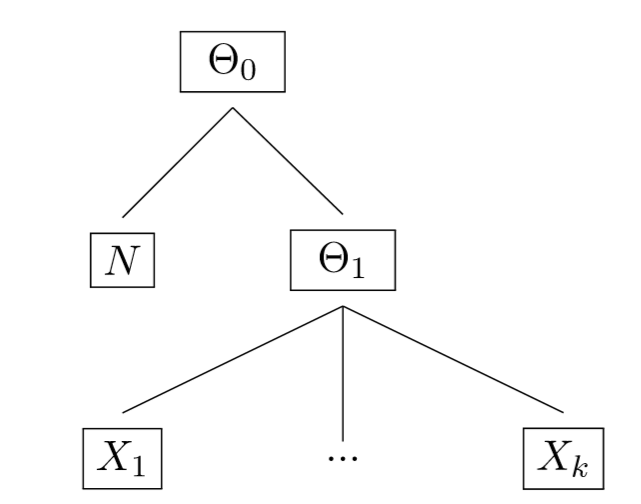
\includegraphics[height=5cm]{Hierarchie}
		\renewcommand{\figurename}{Illustration}
		\caption{Arbre hiérarchique à un niveau.} \label{graph_hierarchie}
	\end{figure}

	Ici, $\Theta_0$ représente une variable aléatoire définie sur $\mathbb{N}_+$ qui sert à créer un lien de dépendance entre la variable $N$ et les $\{X_i, i=1,\dots , k\}$. Ensuite, on a $\theta_1 = \sum_{i=1}^{\theta_0} B_i$ qui sert à créer un lien de dépendance entre les $X_i$. Les $B_i$ sont i.i.d. et indépendants de $\theta_0$. $B_i$ peut appartenir à $R_+$ comme à $N_+$. \\
	
	Sous cette représentation, on obtient une copule archimédienne hiérarchique s'exprimant comme
	
	\begin{equation}
	C(u_0, u_1, \dots, u_n) =
		\mathscr{L}_{\theta_0} \left(
			\mathscr{L}_{\theta_0}^{-1}(u_0) - \ln \left( 
				\mathscr{L}_B  \left(
					\sum_{i=1}^{n} \mathscr{L}_{B}^{-1} \left(
					 \exp \left(
					  - \mathscr{L}_{\theta_0}^{-1}(u_i) 
					  \right) \right)\right)\right)\right),
	\end{equation}
	où $\mathscr{L}$ correspond à la transformée de Laplace d'une variable aléatoire.\\
	
	À ce point-ci, afin de trouver les paramètres d'une telle copule, il suffit d'appliquer \eqref{densite_composee} et \eqref{logLikelyhood_neg}.
	
	\section{Résultats}
	La présente section explique les scénarios testés ainsi que les résultats obtenus avec la méthodologie expliquée dans la section \ref{sect_Maxlikelyhood}.\\
	
	Pour les fins du présent travail, les estimations sont faites sur des données simulées. Pour faire ces simulations, le module \texttt{R} nommé \texttt{copula} \footnote{https://cran.r-project.org/web/packages/copula/copula.pdf}
	offre une fonction \texttt{rCopula} avec laquelle, il est possible de simuler différentes copules connues, dont la copule de Clayton. \\
	
	Pour les copules archimédiennes hiérarchique, le module \texttt{nCopula} \footnote{https://cran.r-project.org/web/packages/nCopula/nCopula.pdf} offre une fonction nommée \texttt{rcompcop}.
	
	\subsection{Copule de Clayton}
	\paragraph{Binomial:}Pour débuter gentiment, prenons un modèle binomial-exponentiel avec une copule de Clayton dont la représentation est exprimée en \eqref{Copule_Clayton}.
	Soient $N \sim Binom(n,q)$ et $X_i \sim X \sim Exp(\beta)$, un sommaire des données simulées aux fins de l'estimation sont présentées dans le tableau \ref{tbl_sommaire_Clayton_Binom}.
	
	% latex table generated in R 3.6.0 by xtable 1.8-4 package
	% Mon Jun 10 14:46:22 2019
	\begin{table}[ht]
		\centering
		\begin{tabular}[width=\textwidth]{llllll}
			\hline
			       $N$ &       $X_1$ &       $X_2$ &             \\ 
			\hline
			Min.   :0.000   & Min.   :  0.0046   & Min.   :   0.0035      \\ 
			1st Qu.:1.000   & 1st Qu.: 28.5104   & 1st Qu.:  28.2379      \\ 
			Median :2.000   & Median : 68.3689   & Median :  68.8120      \\ 
			Mean   :2.001   & Mean   :100.8227   & Mean   : 100.1348      \\ 
			3rd Qu.:3.000   & 3rd Qu.:139.9337   & 3rd Qu.: 136.6506      \\ 
			Max.   :5.000   & Max.   :997.1353   & Max.   :1186.4911      \\ 
			\hline
		\end{tabular}
		%
		\begin{tabular}[width=\textwidth]{lll}
			\hline
			       $X_3$ &       $X_4$ &       $X_5$ \\ 
			\hline
			 Min.   :  0.0032   & Min.   :   0.0035   & Min.   :  0.0028   \\ 
			 1st Qu.: 28.5687   & 1st Qu.:  28.2418   & 1st Qu.: 28.7874   \\ 
			 Median : 68.7141   & Median :  68.1072   & Median : 68.0692   \\ 
			 Mean   : 99.0552   & Mean   : 100.5849   & Mean   :100.6532   \\ 
			 3rd Qu.:136.9080   & 3rd Qu.: 138.4138   & 3rd Qu.:139.0188   \\ 
			 Max.   :857.5771   & Max.   :1026.7730   & Max.   :952.8392   \\ 
			\hline
		\end{tabular}
	\caption[Sommaire des données simulées pour la copule de Clayton avec une loi de fréquence binomiale.]{Sommaire des données simulées pour la copule de Clayton avec $N \sim Bin(5, 2/5),\ X\sim Exp(1/100)$.}
	\label{tbl_sommaire_Clayton_Binom}
	\end{table}

	Du tableau \ref{tbl_sommaire_Clayton_Binom}, on voit que la moyenne du nombre de sinistres est de 2 et que la moyenne des $x_i$ est très proche de 100; ce qui correspond aux attentes.
	De plus, les quantiles des $X_i$ sont très proches l'un de l'autre; ce qui signifie que l'adéquation des variables simulées est bonne. \\
	
	Visuellement parlant, l'illustration \ref{graph_densite_Binom} présente l'adéquation des données empiriques avec les lois théoriques.

	\begin{figure}[H]
	\begin{subfigure}[l]{0.5\textwidth}
		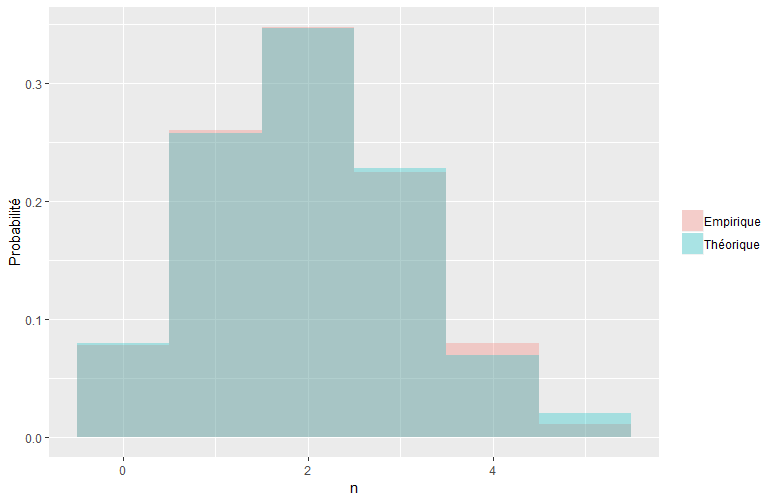
\includegraphics[width=\textwidth]{Graph/Clayton_Binom_N.png}
		\caption{Fréquence}
	\end{subfigure}
	%
	\begin{subfigure}[r]{0.5\textwidth}
		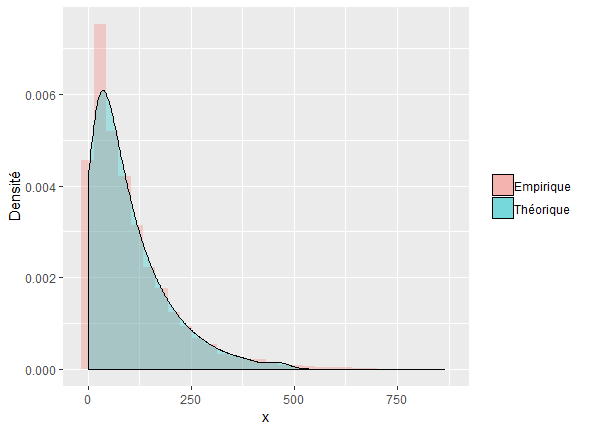
\includegraphics[width=\textwidth]{Graph/Clayton_Binom_X.png}
		\caption{Sévérité}
	\end{subfigure}
	\caption{Comparaisons de la distribution des données simulées avec les distributions théoriques.}
	\label{graph_densite_Binom}
	\end{figure}
	
	On voit donc que les variables simulées ont un comportement très similaire à la distribution marginale théorique des variables.\\
	
	Pour ce qui est du comportement entre les variables, l'illustration \ref{gaph_scatterplot_Binom} présente les nuages de points des variables simulées afin de voir les corrélations.
	
	\begin{figure}[H]
		\centering
		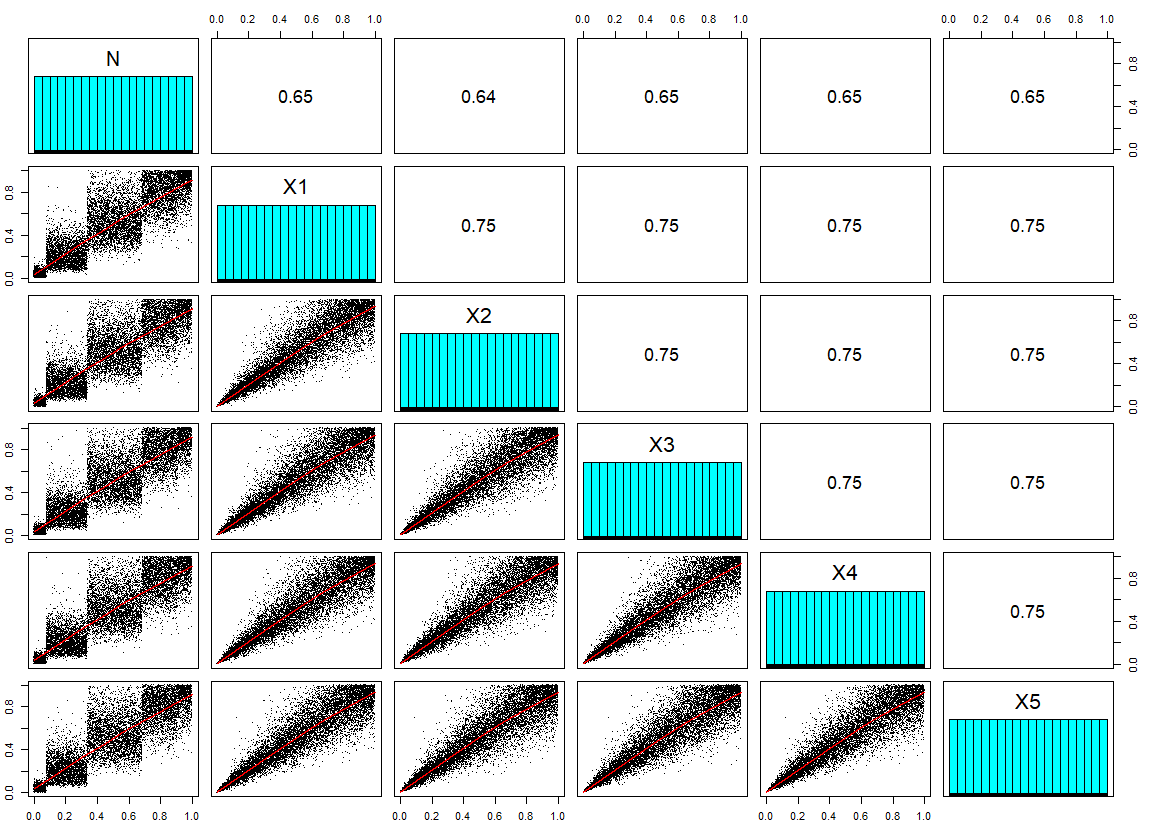
\includegraphics[height=8cm]{Graph/scatterplot_Binom.png}
		\caption[Nuage de points avec copule de Clayton, $N\sim Pois(1)$ et $X\sim Exp(1/100)$]{Nuage de points avec copule de Clayton, $N\sim Pois(1)$ et $X\sim Exp(1/100)$: \\
			En bas de la diagonale se trouve les nuages de points illustrant la corrélation des différentes variables. En haut, se trouve les coefficients de corrélation de Spearman.} 
		\label{gaph_scatterplot_Binom}
	\end{figure}
	

	
	Avec ces résultats, on voit que ...
	
	
	
	
	Avec les données simulées, on désire maintenant estimer les paramètres. 
	les résultats obtenus pour ce scénario sont affichées dans le tableau \ref{tbl_Clayton_Binom}.
	
	% latex table generated in R 3.6.0 by xtable 1.8-4 package
	% Mon Jun 10 14:54:45 2019
	\begin{table}[H]
		\centering
		\begin{tabular}{rrrr}
			\hline
			& q & beta & alpha \\ 
			\hline
			Estimateurs & 0.4024 & 0.0099 & 5.9543 \\ 
			Vrais paramètres & 0.4000 & 0.0100 & 6.0000 \\ 
			\hline
		\end{tabular}
		%
		\begin{tabular}{rr}
			\hline
			&  \\ 
			\hline
			temps de dérivation & 4.22 \\ 
			temps d'estimation & 174.25 \\ 
			\hline
		\end{tabular}
		\caption[Estimations avec une copule de Clayton et $N\sim Binomiale$]{Résultats de l'estimation des paramètres avec une copule de Clayton, $N\sim Binom(n,q)$ et $X \sim Exp(\beta)$ suite à 10\,000 simulations.} \label{tbl_Clayton_Binom}
	\end{table}
	
	\paragraph{Poisson:}Suite aux résultats concluants du premier exemple, un modèle avec $N \sim Pois(\lambda)$ peut ajouter un défi en terme de temps de calcul puisque cette loi a un support pouvant atteindre de grands nombres. Soient $N \sim Pois(\lambda)$ et $X_i \sim X \sim Exp(\beta)$, un sommaire des données simulées aux fins de l'estimation sont présentées dans le tableau \ref{tbl_sommaire_Clayton_Pois_1}.
	
	% latex table generated in R 3.6.0 by xtable 1.8-4 package
	% Mon Jun 10 10:40:57 2019
	\begin{table}[H]
		\centering
		\begin{tabular}{lllll}
			\hline
			       $N$ &      $X_1$ &      $X_2$ &       $X_3$ &       $X_4$ \\
			\hline
			 Min.   :0.0000   & Min.   :   0.0093   & Min.   :  0.012   & Min.   :  0.0129   & Min.   :   0.0172 \\
			 1st Qu.:0.0000   & 1st Qu.:  29.7317   & 1st Qu.: 29.593   & 1st Qu.: 29.4194   & 1st Qu.:  29.5410 \\
			 Median :1.0000   & Median :  70.2592   & Median : 70.060   & Median : 70.3962   & Median :  70.1612 \\
			 Mean   :0.9989   & Mean   : 101.2211   & Mean   :101.325   & Mean   :100.4977   & Mean   : 101.1802 \\
			 3rd Qu.:2.0000   & 3rd Qu.: 140.8462   & 3rd Qu.:141.488   & 3rd Qu.:136.6166   & 3rd Qu.: 139.6666 \\
			 Max.   :6.0000   & Max.   :1003.4804   & Max.   :884.530   & Max.   :875.3387   & Max.   :1071.0681 \\
			\hline
		\end{tabular}

		\begin{tabular}{llll}
			\hline
			$X_5$ &      $X_6$ &       $X_7$ &       $X_8$ \\ 
			\hline
			Min.   :   0.0121   & Min.   :  0.0118   & Min.   :  0.01   & Min.   :   0.0105   \\ 
			1st Qu.:  29.3078   & 1st Qu.: 29.7289   & 1st Qu.: 29.23   & 1st Qu.:  29.6958   \\ 
			Median :  70.1336   & Median : 70.0210   & Median : 70.47   & Median :  70.2837   \\ 
			Mean   : 100.2858   & Mean   :100.6869   & Mean   :100.69   & Mean   : 100.3833   \\ 
			3rd Qu.: 137.5781   & 3rd Qu.:138.3483   & 3rd Qu.:136.65   & 3rd Qu.: 138.1448   \\ 
			Max.   :1089.6821   & Max.   :952.6193   & Max.   :810.01   & Max.   :1029.2935   \\ 
			\hline
	\end{tabular}
	\caption[Sommaire des données simulées pour la copule de Clayton avec une loi de fréquence Poisson.]{Sommaire des données simulées pour la copule de Clayton avec $N \sim Pois(1),\ X\sim Exp(1/100)$.}\label{tbl_sommaire_Clayton_Pois_1}
	\end{table}

	L'illustrations \ref{graph_densite_Poisson_1} compare la distribution des données simulées avec celle des lois théorique.
	
	\begin{figure}[H]
		\begin{subfigure}[l]{0.5\textwidth}
			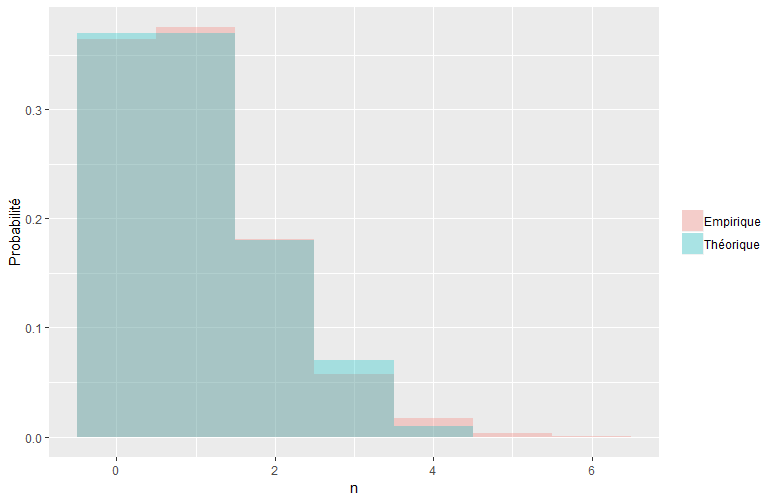
\includegraphics[width=\textwidth]{Graph/Clayton_Poiss_1_N.png}
			\caption{Fréquence}
		\end{subfigure}
		%
		\begin{subfigure}[r]{0.5\textwidth}
			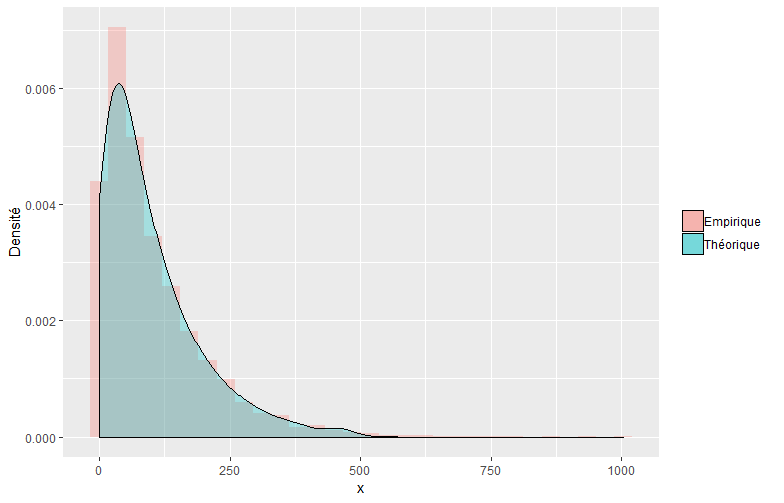
\includegraphics[width=\textwidth]{Graph/Clayton_Poiss_1_X.png}
			\caption{Sévérité}
		\end{subfigure}
		\caption{Comparaisons de la distribution des données simulées avec les distributions théoriques.}\label{graph_densite_Poisson_1}
	\end{figure}

	L'illustration \ref{gaph_scatterplot_Poiss_1} présente les nuages de points des variables simulées afin de voir les corrélations.

	\begin{figure}[H]
		\centering
		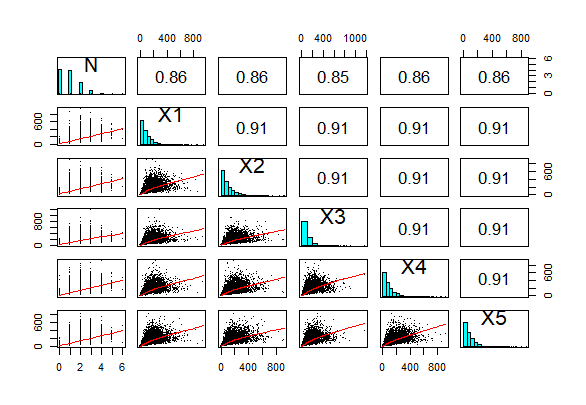
\includegraphics[height=8cm]{Graph/scatterplot_Poisson_1.png}
		\caption[Nuage de points avec copule de Clayton, $N\sim Pois(1)$ et $X\sim Exp(1/100)$]{Nuage de points avec copule de Clayton, $N\sim Pois(1)$ et $X\sim Exp(1/100)$: \\
			En bas de la diagonale se trouve les nuages de points illustrant la corrélation des différentes variables. En haut, se trouve les coefficients de corrélation de Spearman.} 
		\label{gaph_scatterplot_Poiss_1}
	\end{figure}
	
	Les résultats obtenus sont présentés dans le tableau \ref{tbl_Clayton_Poisson}.
	
	% latex table generated in R 3.6.0 by xtable 1.8-4 package
	% Thu Jun 06 16:25:40 2019
	\begin{table}[H]
		\centering
		\begin{tabular}{rrrr}
			\hline
			& lambda & beta & alpha \\ 
			\hline
			Estimateurs & 1.0006 & 0.0099 & 5.9160 \\ 
			Vrais paramètres & 1.0000 & 0.0100 & 6.0000 \\ 
			\hline
		\end{tabular}
%	
	\begin{tabular}{rr}
		\hline
		&  \\ 
		\hline
		temps de dérivation & 13.29 \\ 
		temps d'estimation & 86.24 \\ 
		\hline
	\end{tabular}
		\caption[Estimations avec une copule de Clayton et $N\sim Poisson$]{Résultats de l'estimation des paramètres avec une copule de Clayton, $N\sim Pois(\lambda)$ et $X \sim Exp(\beta)$ suite à 10\,000 simulations.}\label{tbl_Clayton_Poisson}
	\end{table}

	Lorsque $N \sim Poisson(2)$, le temps de calcul dépasse trente minutes puisque le 99,9999 percentile de cette loi est de 12. Ainsi la méthode du maximum de vraisemblance nécessite de générer une liste de douze fonctions qui sont dérivées jusqu'à douze fois. Même avec la fonction \texttt{Deriv} de \texttt{R}, ce processus est extrêmement long.\\
		
	Ce que l'on peut observer avec ces deux résultats, c'est, d'une part, qu'avec 10\,000 simulations, on obtient des résultats très adéquats. Cependant, il faut soulever que les valeurs de départ pour l'optimisation de la fonction de vraisemblance sont les véritables valeurs; ce qui peut faire en sorte que les valeurs sont plus précises qu'elles ne l'auraient été si les valeurs de départ avaient été autre. D'autre part, on peut observer que le temps de calcul augmente significativement si $N$ peut prendre des valeurs supérieures à 5 et si le nombre de paramètres à estimer est grand.

	\subsection{Copule archimédienne hiérarchique}
	Désormais, prenons la copule qui nous intéresse vraiment: la copule archimédienne hiérarchique. Avec $\theta_0 \sim logarithmique\left(\gamma = 1-\exp(-\alpha_0)\right)$, $B \sim Gamma(1/\alpha_1, 1)$, $N \sim Binom(5,q)$ et $X_i \sim X \sim Exp(\beta)$ on obtient les résultats présentés dans le tableau \ref{tbl_archi_hierar}.
	\begin{table}[H]
		\centering
		\begin{tabular}{rrrrr}
			\hline
			& $\alpha_{0}$ & $\alpha_{1}$ & $\beta$ & $q$ \\ 
			\hline
			Estimateurs & 0.50 & 5.17 & 0.01 & 0.40 \\ 
			Vrais Paramètres & 0.50 & 5.00 & 0.01 & 0.40 \\ 
			\hline
			Temps de calcul & 821.4 sec. \\
			\hline
		\end{tabular}
		\caption[Estimations avec une copule archimédienne hiérarchique et $N\sim Binomiale$]{Résultats de l'estimation des paramètres avec une copule archimédienne hiérarchique, $N \sim Binomiale(5, q)$ et $X \sim Exp(\beta)$ suite à 10\,000 simulations.} \label{tbl_archi_hierar}
	\end{table}

	Dans cet exemple, on note que le temps de calcul est significativement supérieur à celui présenté dans le tableau \ref{tbl_Clayton_Binom}. Ce phénomène est explicable du fait qu'il y a plus de paramètres à estimer et que la copule contient plusieurs fonctions imbriquées qui nécessitent plus d'étapes dans le processus de dérivation en chaîne.
	
	\section{Conclusion}
	Pour conclure, le modèle collectif du risque présenté dans \cite{Itre5} présente un défi dans l'estimation des paramètres par la méthode du maximum de vraisemblance tel que présentée dans la section \ref{sect_Maxlikelyhood} puisque la dérivation en chaîne sur un grand nombre de variables pose un problème de temps de calcul.\\
	
	 À cet effet, une solution envisageable pourrait être d'utiliser la vraisemblance par décomposition hiérarchique proposé dans \cite{LikelyhoodEstimation} afin de trouver le paramètre de dépendance entre $N$ et $X_1$, puis de se limiter à un nombre restreint de $X_i$ (disons 5) afin d'estimer le paramètre de dépendance entre les $X_i$. Cependant, avec cette méthode le fait de travailler avec des variables continues et discrètes peut causer un problème. Pour ce qui est de trouver les paramètres des lois de $N$ et $X$, la méthode du maximum de vraisemblance classique (de façon univariée) pourrait être envisagée.
 
	
	\clearpage
	\bibliography{BibRRT_Presentation_2019-05-31.bib}
	\bibliographystyle{apalike}

\end{document}
 